\documentclass{report}
\usepackage[utf8]{inputenc}
\usepackage{lib/report-template}
\usepackage[all]{background}
\usepackage{lipsum}

\usepackage{titlesec}
\titleformat{\chapter}
  {\normalfont\LARGE\bfseries}{\thechapter}{1em}{}
\titlespacing*{\chapter}{0pt}{3.5ex plus 1ex minus .2ex}{2.3ex plus .2ex}

\SetBgContents{}% Set contents
\SetBgPosition{-0.5cm,-5.0cm}% Select location
\SetBgOpacity{1.0}% Select opacity
\SetBgAngle{90.0}% Select rotation of logo
\SetBgScale{2.0}% Select scale factor of logo


%Line spacing
\renewcommand{\baselinestretch}{1.5}

\title{projeto ATLAS}

\date{August 2019}


\begin{document}

\begin{titlepage}.
    \begin{tikzpicture}[remember picture,overlay]

% UTT Background under the title and info box
\coordinate [right=8mm, below=65mm] (uttbackground_anchor) at (current page.north west);
\node [name=uttsquare,anchor=north west] at (uttbackground_anchor){
%\includegraphics[width=19.4cm]{first-page-background.png}};
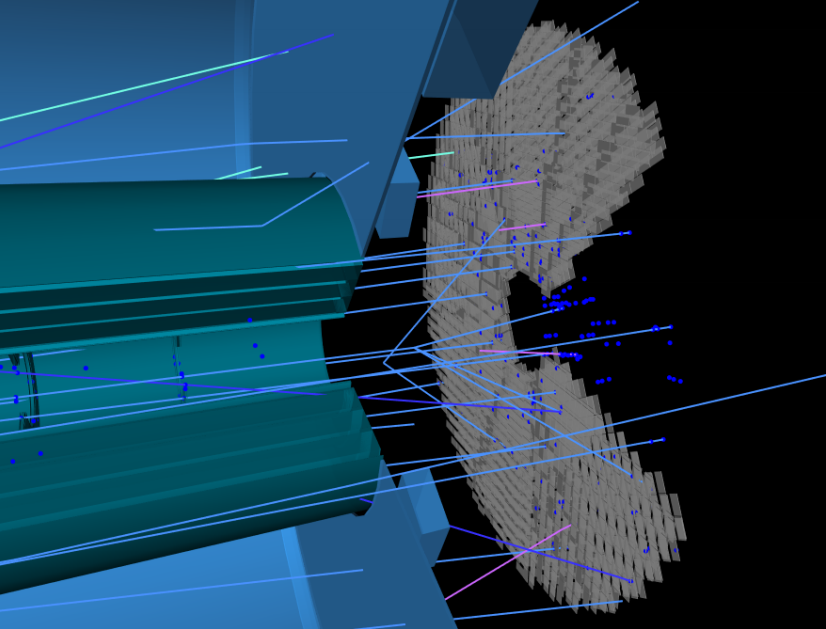
\includegraphics[width=19.4cm]{assets/ATLAS_BACKGROUND.png}};

\end{tikzpicture}

    % Margin to begin the text under the uttsquare
    \vspace{3.5cm}

    % Internship title
    
    \begin{textblock*}{15cm}(3cm,2cm)
        \begin{Huge}
            \begin{center}
                \makeatletter
                \noindent\textcolor{black}{Projeto de pesquisa de pós-doutorado em física}
                \makeatother
            \end{center}
        \end{Huge}
    \end{textblock*}
    
    % project tipe
    \begin{textblock*}{15cm}(2.5cm,5.5cm)
        \makeatletter
        \begin{LARGE}
            \begin{center}
                \color{black}
                {\it  }\\
            \end{center}
         \end{LARGE}
     
    \end{textblock*}
    
    %TITLE
    \begin{textblock*}{15cm}(3cm,12cm)
        \begin{Huge}
            \begin{center}
                \makeatletter
                \noindent\textcolor{white}{\textbf{Desenvolvimento de um detector de silício para a medida de trajetórias e tempo no experimento ATLAS-LHC}}
                \makeatother
            \end{center}
        \end{Huge}
    \end{textblock*}

    % Author
    \begin{textblock*}{15cm}(2.5cm,22cm)
        \begin{LARGE}
        \begin{center}
            \color{black}
                \textbf{Autor :} Dr. Renato Aparecido Negrão de Oliveira \\  \\ 
        \end{center}
            
        \end{LARGE}
        
    \end{textblock*}
    
    % FOOT NOTE
    \begin{textblock*}{15cm}(3cm,25cm)
        \makeatletter
        \begin{center}
            {\color{black}
                \textbf{SÃO PAULO, 2020} 
            }
        \end{center}
        \makeatother
    \end{textblock*}

\end{titlepage}

\begin{titlepage}.
    \begin{tikzpicture}[remember picture,overlay]

% UTT Background under the title and info box
\coordinate [right=8mm, below=65mm] (uttbackground_anchor) at (current page.north west);
\node [name=uttsquare,anchor=north west] at (uttbackground_anchor){
%\includegraphics[width=19.4cm]{first-page-background.png}};
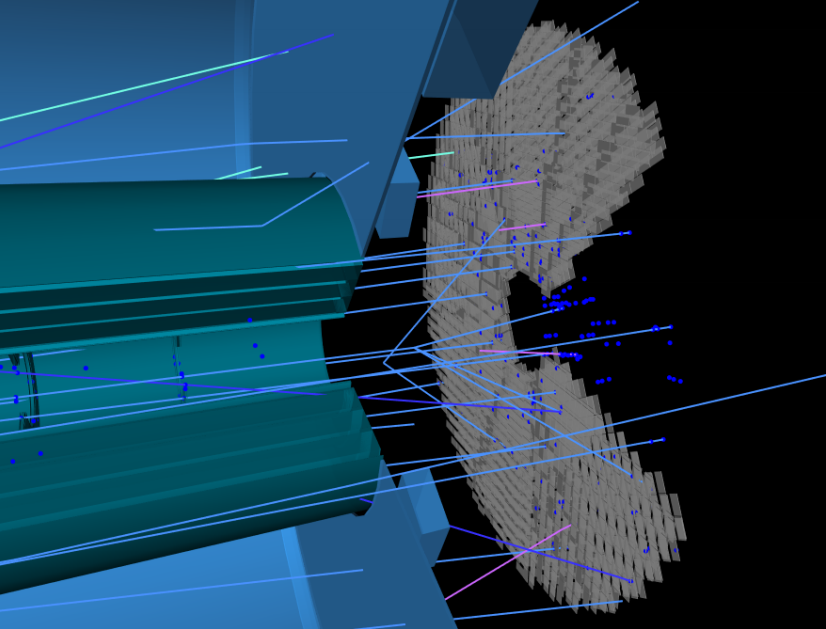
\includegraphics[width=19.4cm]{assets/ATLAS_BACKGROUND.png}};

\end{tikzpicture}

    % Margin to begin the text under the uttsquare
    \vspace{3.5cm}

    
    % Authhor
    \begin{textblock*}{15cm}(3cm,2.cm)
        \makeatletter
        \begin{huge}
            \begin{center}
                \color{black}
                 Renato Aparecido Negrão de Oliveira\\ 
            \end{center}
         \end{huge}
     
    \end{textblock*}
    
    %TITLE
    \begin{textblock*}{15cm}(3cm,12cm)
        \begin{Huge}
            \begin{center}
                \makeatletter
                \noindent\textcolor{white}{\textbf{Desenvolvimento de detectores de silício para a medida de trajetórias e tempo no experimento ATLAS-LHC}}
                \makeatother
            \end{center}
        \end{Huge}
    \end{textblock*}

    % Info box
    \begin{textblock*}{15cm}(2.5cm,22cm)
        \makeatletter
        \begin{LARGE}
            \setcellgapes{4pt}
            \makegapedcells
            {\color{black}\begin{tabularx}{15cm}{XX}
                \textbf{Supervisor :} Dr. Stefan Guindon
(CERN, EP-Department)\\ 
                \textbf{Co-Supervisor :} Dr. 
Marco Aurelio Lisboa Leite (IF-USP)
            \end{tabularx}}
        \end{LARGE}
        \makeatother
    \end{textblock*}
    
    % FOOT NOTE
    \begin{textblock*}{15cm}(3cm,25cm)
        \makeatletter
        \begin{center}
            {\color{black}
                \textbf{SÃO, PAULO 2020} 
            }
        \end{center}
        \makeatother
    \end{textblock*}

\end{titlepage}


\chapter*{Resumo}

%A necessidade de desenvolver detectores semicondutores rápidos para a medida de trajetória de partículas carregadas no {\it Large Hadron Collider} (LHC) tem aumentado no decorrer da última década em resposta ao aumento da luminosidade do feixe produzido no LHC.

Com o aumento da luminosidade do feixe produzido no LHC, o qual será três vezes maior após o seu upgrade \cite{HL_LHC,tdr}, vários desafios experimentais são colocados para os experimentos, dentre eles está a reconstrução do grande número de eventos que ocorrem durante o cruzamento dos pacotes do feixe no ponto de interação no LHC, o que provoca o empilhamento desses eventos.
Em vista disso, uma forma de abordar os efeitos do empilhamento das colisões e mitigar esse problema, é através do uso de técnicas de medida de tempo com alta precisão para distinguir as colisões que não podem ser separadas espacialmente. 

Para solucionar esse problema, um novo sistema de detecção será construído - denominado {\it High Granularity Timing Detector} (HGTD) - para a fase-II do experimento ATLAS, o qual é baseado em sensores semicondutores de silício com ganho intrínseco para a multiplicação de cargas
%e cuja tecnologia empregada permite operá-los em um regime de baixo ganho de carga 
({\it Low Gain Avalanche Detector} - LGAD). Esse detector será instalado na região frontal do experimento, cobrindo o intervalo em pseudo-rapidez de $2.4< |\eta| <4.0$, e permitirá medir intervalos de tempo com resolução da ordem de 20-30 pico segundos.

%Por conseguinte, a medida precisa do tempo irá melhorar a reconstrução do vértice da colisão, tendo em vista que diminui as incertezas na associação das trajetórias ao vértice onde foram originadas, possibilitando o aumento significativo do desempenho, e permitindo reconstruir jatos de partículas com grande precisão. A melhoria na capacidade de reconstrução de jatos - que será obtida com o HGTD - aumentará a sensibilidade do experimento permitindo explorar observáveis antes não explorados devido aos limites experimentais.

À vista disso, neste projeto de pós-doutorado é proposto o desenvolvimento de atividades de pesquisa em colaboração com o experimento ATLAS no CERN. O trabalho será focado na pesquisa e desenvolvimento de sistemas utilizando sensores semicondutores do tipo LGAD visando aplicações que requerem grande tolerância à altos níveis de radiação ionizante \cite{JIN_LGAD,NIMA_LGAD,NIMA_LGAD_I,NIMA_LGAD_II,NIMA_LGAD_III} - com o objetivo de otimizar sua capacidade para utilização no ATLAS. %A consolidação desse tipo de sensores oferece uma grande oportunidade em termos de pesquisa e desenvolvimento na área de sensores semicondutores, com aplicações em diversas áreas da física e tecnologia em geral.


\chapter*{Abstract}

%The development of fast response semiconductor sensor for particle tracking at LHC has increased in the past decade in response to the high luminosity expected for the upgraded Large Hadron Collider (LHC).

The significant increase of the beam luminosity by a factor three \cite{HL_LHC,tdr} is one of the main experimental challenges for the High Luminosity LHC (HL-LHC) physics program, and a new way to mitigate the effects of pile-up is to use high-precision timing information to distinguish between collisions occurring close in space but well-separated in time.

To address this experimental challenge, a High-Granularity Timing Detector (HGTD), based on low gain avalanche detector technology is proposed for the ATLAS Phase-II upgrade. The detector will be installed at the forward region, covering the pseudorapidity range between $2.4< |\eta| <4.0$, and allowing the measurement of the time interval of the order of 20-30 picoseconds.

%The high-precision timing information will greatly improve the track-to-vertex association, leading to a significant increase in performance allowing for a high-precision reconstruction of particle jets. These improvements in jet reconstruction performance will translate into important sensitivity gains and enhance the reach of the ATLAS physics program.

Therefore, in this project, it is proposed to be performed activities on research and development in collaboration with ATLAS experiment at CERN. The research will be focused on the development of the LGDA sensors - recently developed to operate at higher levels of radiation dose \cite{JIN_LGAD,NIMA_LGAD,NIMA_LGAD_I,NIMA_LGAD_II,NIMA_LGAD_III} - in order to optimize the device capabilities to operate in the ATLAS experiment. %The consolidation of this type of sensors offers a unique opportunity for research and development regarding the semiconductor sensors, with a great spin-off for other areas of physics and general technology.

\tableofcontents

% Conteudo do capitulo
%1- Razoes fisicas para se ter o ATLAS UPGRADE 
%2- Porque a melhor escolha para o upgrade e o LGAD
%3- Importacia cientifica do LGAD
%4- Introducao ao LGAD
%5- Proposta do projeto
%6- Alguns detalhes sobre o escopo do projeto
%7- Importancia para o grupo 
\chapter{Introdução}

Na última década, o experimento ATLAS no LHC foi extremamente importante, fornecendo informações sobre as propriedades do bóson de Higgs e contribuindo para valiosas descobertas no campo da física nuclear e de partículas \cite{atlas_rev}. Tendo em mente esse grande legado para a física, atualmente o experimento ATLAS, e o LHC, estão se preparando para iniciar uma nova etapa na pesquisa científica com o objetivo de atingir níveis de sensibilidade e precisão nas medidas que vão muito além dos níveis atuais \cite{tdr}, e cobrir áreas de pesquisa importantes, ainda não exploradas, no contexto do modelo padrão (SM), propriedades do bóson de Higgs e a busca por assinaturas físicas que estão além do modelo padrão.

Diversas medidas feitas para estudar o modelo padrão, bem como as propriedades do bóson de Higgs, são limitadas por incertezas sistemáticas presentes nos dados. Dessa forma é importante que os detectores sejam capazes de diminuir essas incertezas relacionadas com a reconstrução dos objetos físicos - e.g. jatos de partículas - e com a modelagem do fundo presente nos eventos reconstruídos. Com esse objetivo, melhorias na razão sinal-fundo e o aumento da estatística dos dados são necessárias para aumentar a precisão dos observáveis físicos. %Neste contexto, o \textit{High Granularity Timing Detector} (HGTD) será um detector importante para a melhoria na reconstrução de objetos físicos na região frontal do experimento ATLAS, permitindo alcançar níveis de precisão similares aos obtidos para a região de pseudo-rapidez central. Isso permitira reduzir substancialmente o erro sistemático nesse espaço de fase, e explorar com grande precisão os fenômenos físicos nessa região.

% 1 - Razoes físicas para se ter o ATLAS UPGRADE 
Neste contexto, para o experimento ATLAS, um dos desafios experimentais é reconstruir partículas na região de rapidez frontal, produzidas na interação inicial, de modo a associá-las corretamente com o vértice onde foram originadas, em um regime de altas taxas de colisão. Para solucionar esse desafio, um novo sistema de detecção frontal, denominado HGTD ({\it High Granularity Timing Detector}), está sendo desenvolvido - com base nos sensores LGAD ({\it Low Gain Avalanche Detector}) - para fornecer uma medida precisa de tempo, com o objetivo de diminuir as incertezas experimentais na reconstrução dos eventos, e fornecer uma precisão na medida similar ao obtido para a região de pseudo-rapidez central \cite{tdr}.

Como ilustra a Fig. \ref{hgtd}, o HGTD foi desenhado para ser instalado na região frontal do experimento, em ambos os lados a uma distancia de $3.5m$ do ponto de interação do feixe, região a qual está localizada após o volume do ATLAS {\it Inner Tracker} (ITk) \cite{tdr}.

\thispagestyle{plain}
Com o aumento significativo da precisão na medida de partículas frontais, através do uso do HGTD, será possível medir com precisão a luminosidade do feixe, a qual é uma medida crítica para a determinação da seção de choque da produção de partículas em diversas analises físicas, além de  permitir a reconstrução de jatos de partículas com grande precisão. A melhoria na capacidade de reconstrução de jatos - que será obtida com o HGTD - aumentará a sensibilidade do experimento, permitindo explorar observáveis antes não explorados devido aos limites experimentais \cite{tdr}.

\thispagestyle{plain}
\begin{figure} 
    \centering
    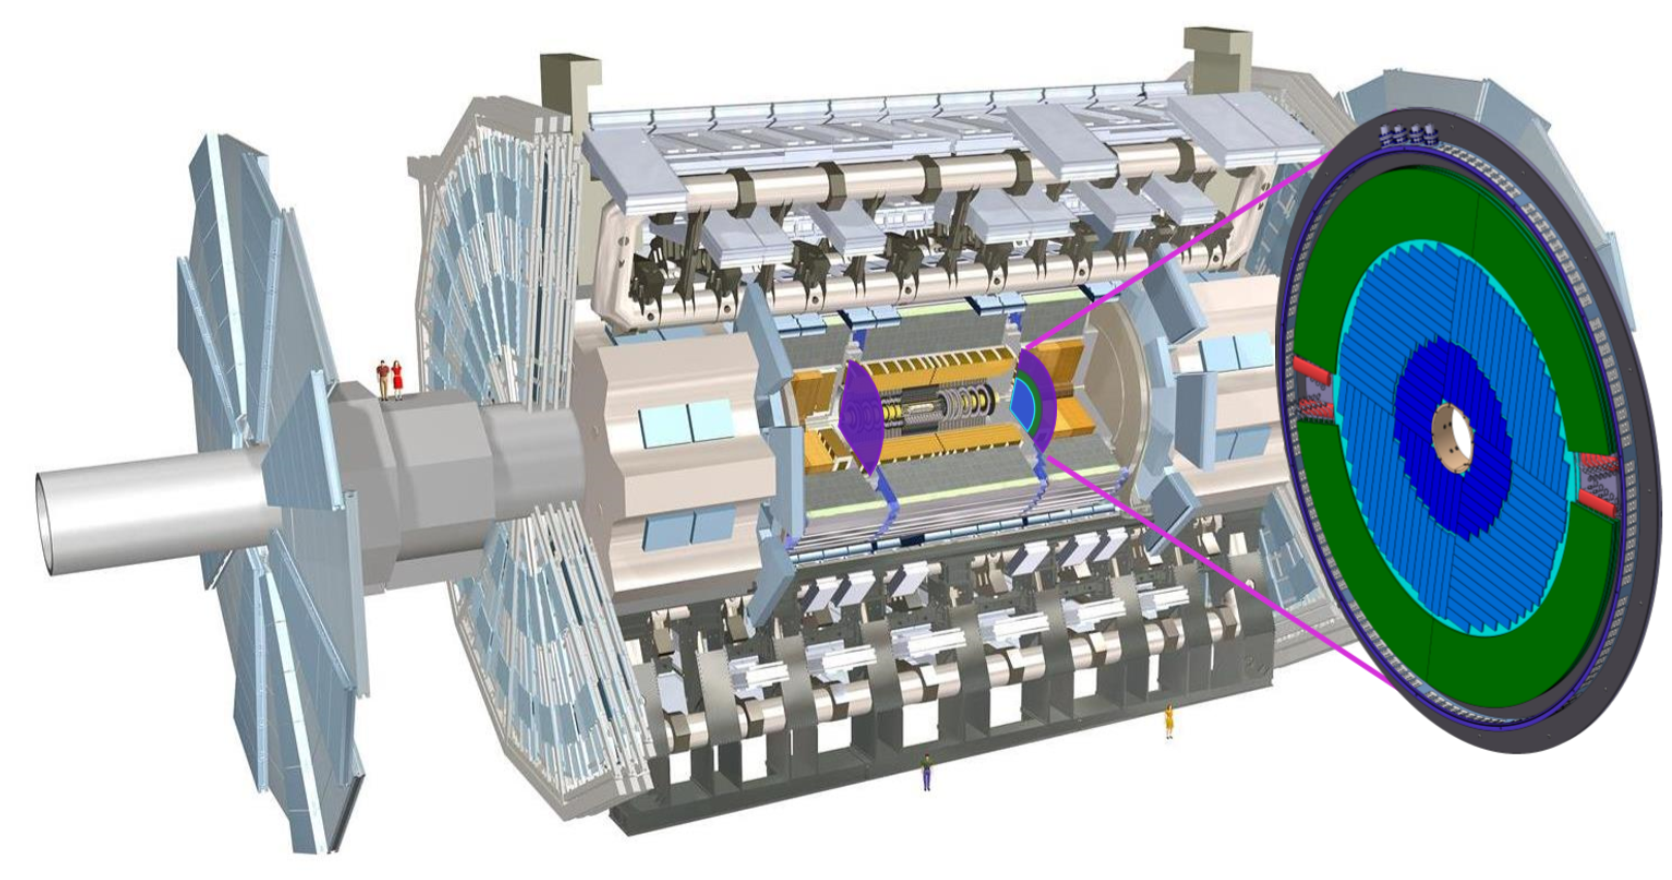
\includegraphics[width=15.0cm]{assets/ATLAS_HGTD.png}
    \caption{ Figura mostrando em detalhes a posição onde o HGTD será instalado. A figura também mostra o experimento ATLAS e os seus vários sistemas.}
    \label{hgtd}
\end{figure}

% 5 - PROPOSTA DO PROJETO
A vista disso, o propósitos deste projeto é desenvolver técnicas e metodologias experimentais necessárias para a caracterização física de sensores semicondutores do tipo LGAD para o upgrade do experimento ATLAS no CERN, bem como participar na construção do primeiro protótipo do HGTD.

\section{O sensor LGAD}

O sensor LGAD foi adotado como base tecnológica para a construção do HGTD por apresentar excelentes características com respeito ao compromisso entre ganho e resolução temporal \cite{tdr,JIN_LGAD,NIMA_LGAD,NIMA_LGAD_I,NIMA_LGAD_II,NIMA_LGAD_III}. Além da resposta rápida à incidência de radiação, esse tipo de sensor possui ganho intrínseco devido ao perfil de dopagem empregado no material semicondutor, o que torna possível amplificar o sinal produzido e dessa forma operá-lo em modo de avalanche de carga \cite{JIN_LGAD,NIMA_LGAD,NIMA_LGAD_I,NIMA_LGAD_II,NIMA_LGAD_III}. Essas características comprovam a importância dessa tecnologia para o desenvolvimento da próxima geração de sensores semicondutores para aplicações que requerem altas taxas de contagem e ganho moderado.
\thispagestyle{plain}

Como ilustra a Fig. \ref{lgad}, LGAD são sensores semicondutores planos com ganho intrínseco. O ganho do sensor é determinado pela quantidade de dopante implantado na matriz de silício formando a camada de multiplicação. Como mostra a Fig. \ref{lgad}, sua arquitetura é composta de uma camada de material semicondutor do tipo n sobre uma camada do tipo p, com a adição de uma camada altamente dopada do tipo p localizada entre a junção n-p, cuja função é criar um alto campo elétrico responsável por produzir a avalanche das cargas e amplificar o sinal elétrico. Dessa forma, quando uma partícula atravessa a região sensível do detector, elétrons e lacunas são criados produzindo uma corrente inicial. Os elétrons ao atingirem a região de amplificação produzem novos pares elétron lacuna sendo desse modo multiplicados em um processo de avalanche, produzindo uma corrente de 10 a 30 vezes maior do que a gerada pelas ionizações primárias \cite{JIN_LGAD,NIMA_LGAD_III}. 

\begin{figure}
    \centering
    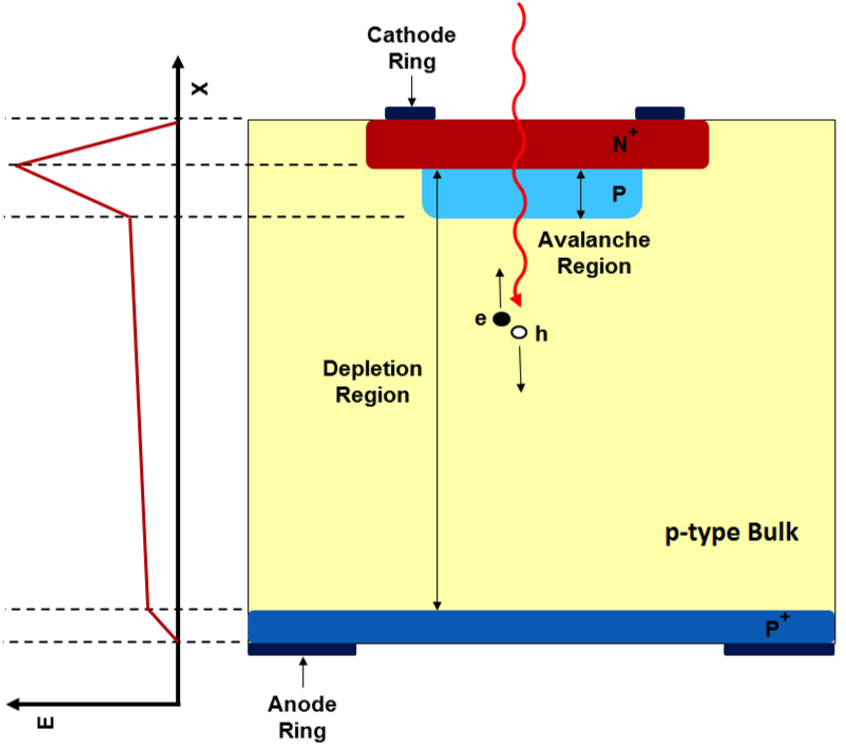
\includegraphics[width=7.0cm]{assets/lgad.png}
    \caption{Figura mostrando a estrutura esquemática de um sensor LGAD.}
    \label{lgad}
\end{figure}
\thispagestyle{plain}

\section{Protótipo do HGTD}

A Fig. \ref{hgtd}.a mostra o módulo híbrido do HGTD composto pelo sensor LGAD, dois ASICs - responsáveis pela aquisição do sinal - que juntamente com o LGAD formam o denominado \textit{bare module}, e as placas de circuito impresso flexível, compostas por duas partes, uma colada permanentemente no \textit{bare module} denominada \textit{Module Flex}, e a outra que se estende ao longo do detector, \textit{Flex Tail}. O sensor LGAD e os ASICs serão conectados através de uma solda de ligação. Todas as conexões entre o ASIC e a eletrônica de aquisição de dados serão feitas através do circuíto impresso flexível, \textit{Module Flex}, onde o ASIC é conectado ao circuíto através de fios soldados entre ambos.    

A Fig. \ref{hgtd}.b mostra o detalhe três módulos colados precisamente sobre a placa de refrigeração e posicionados ao longo da direção z do HGTD. Na figura é possível visualizar os cabos flexíveis, \textit{Flex Tail}, responsáveis por transmitir os sinais do ASIC, e fornecer os serviços de alimentação de baixa tensão, e alta tensão para os sensores. 

Como mostra a Fig. \ref{hgtd}.c, o protótipo do HGTD será composto de uma placa de refrigeração, onde dez módulos serão precisamente colados. A eletrônica de aquisição e leitura dos dados será conectada através dos cabos flexíveis e protótipos das fontes de alimentação de alta e baixa tensão do sistema serão utilizadas. Por fim, serão efetuados testes de funcionamento com a detecção de raios cósmicos e raios-X.    

\begin{figure}
    \centering
    \subfloat[a]{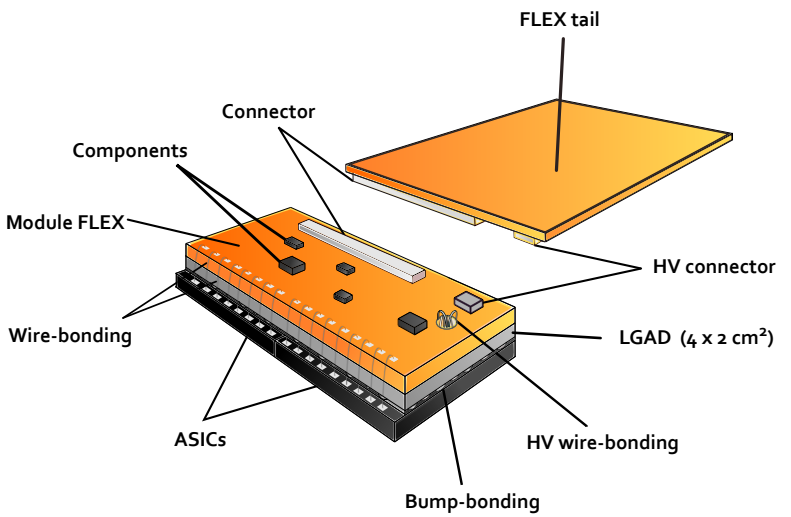
\includegraphics[width=7.0cm]{assets/HGTD_module.png}}
    \subfloat[b]{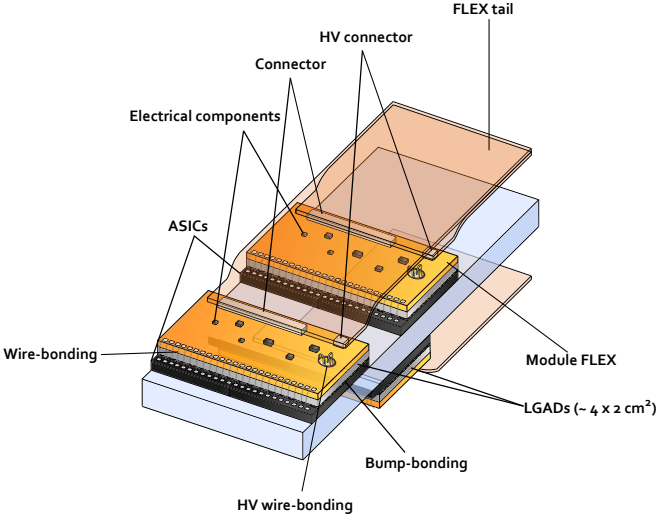
\includegraphics[width=7.0cm]{assets/HGTD_Prototype.png}}
    \subfloat[c]{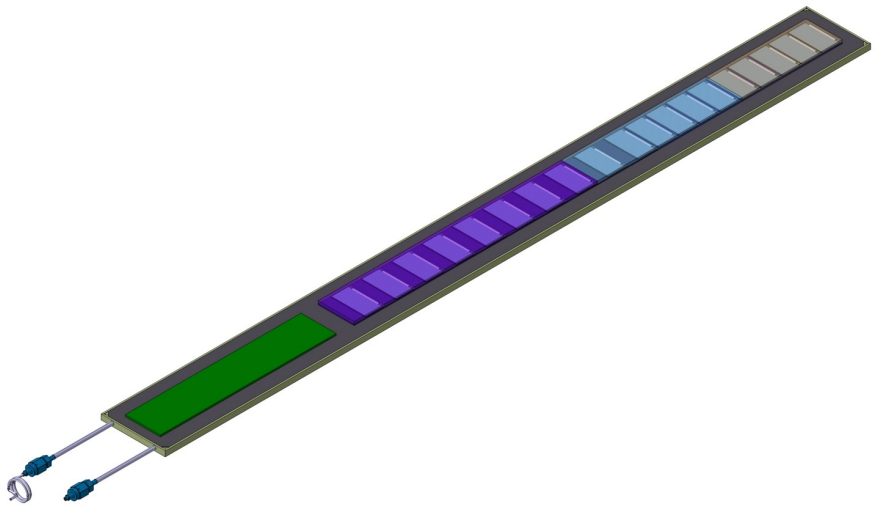
\includegraphics[width=7.0cm]{assets/HGTD_Mec_Module.png}}
    \label{hgtd}
    \caption{Figura mostrando os componentes do HGTD. [a] Módulo híbrido do HGTD. [b] Três módulos colados na placa de refrigeração. [c] Estrutura mecânica da placa de refrigeração.}
\end{figure}
\thispagestyle{plain}
\renewcommand{\cleardoublepage}{}
\renewcommand{\clearpage}{}
% Conteúdo do capitulo 
% 1- Desenvolver e caracterizar sensores LGAD para o upgrade do ATLAS

\chapter{Objetivos do projeto}

% 1 - Descrição do desafio experimental para o ATLAS
O objetivo científico deste projeto é participar do desenvolvimento de um sistema de detecção para a região de pseudo-rapidez frontal que seja capaz de melhorar a precisão da medida de luminosidade do feixe e a reconstrução de partículas no experimento ATLAS, para operar durante a fase de alta luminosidade do LHC ({\it High Luminosity LHC} (HL-LHC)) \cite{HL_LHC,tdr}. 

Para superar esse desafio científico, este projeto concentrar-se-á na pesquisa e desenvolvimento de um sistema de detecção frontal ATLAS-HGTD, cuja a técnica experimental é baseada na medida do tempo de vôo das partículas, medindo intervalos de tempo com resolução da ordem de 20-30ps \cite{tdr}, tornando dessa forma possível associar as partículas ao seu vértice de produção para colisões próton-próton no HL-LHC. Para realizar a construção do HGTD, os sensores do tipo LGAD serão adotados como base tecnológica, tendo em vista que eles apresentam excelentes características com respeito ao compromisso entre ganho e resolução temporal. 
\thispagestyle{plain}

O Detector \textit{High Granularity Timing Detector} (HGTD) é um projeto de atualização de fase II para o detector ATLAS \cite{tdr}. É essencial validar os principais aspectos do detector no CERN em 2021 e 2022 no programa de demonstração. A primeira parte importante do projeto está centrada na validação do desempenho térmico do resfriamento de CO$_{2}$ em uma única linha de leitura usando aquecedores de silício para emular a dissipação de energia dos módulos. Essa validação visa garantir a estabilidade térmica dos módulos HGTD com a placa de resfriamento. Os testes de estabilidade térmica serão realizados no CERN até Outubro de 2021. O pesquisador de pós-doutorado terá papel de liderança nas medições de dissipação de energia e na análise do desempenho térmico dos aquecedores da placa de resfriamento.

Em Outubro de 2021, o foco do projeto do demonstrador mudará para os primeiros módulos completos do HGTD (sensor de silício LGAD + ASIC de interface). Estes serão montados e levados ao CERN, onde serão instalados na placa de resfriamento. O pesquisador participará da montagem dos módulos e PCBs flexíveis que serão montados no CERN. Este procedimento de montagem é uma etapa muito importante para validação do detector, e irá definir o caminho completo de leitura dos sinais dos módulos HGTD para as placas eletrônicas de aquisição periféricas. A cadeia de leitura completa será exercitada e estudada para garantir que uma resolução de tempo de 30ps seja alcançável para o detector no início de 2022.

Além dos módulos para o demonstrador, módulos completos serão testados em campanhas periódicas de teste com feixe na instalação \textit{Super Proton Synchrotron} (SPS) no CERN, quando a instalação reiniciar a execução de prótons em meados de 2021. Durante essas campanhas ao longo de 2022, muitos módulos HGTD serão estudados usando píons de alta energia para entender e validar seu desempenho antes e após a irradiação. O pesquisador participará e concentrará parte de seu tempo no estudo de módulos durante essas campanhas de testes com feixe no CERN. Da mesma forma, o pesquisador também participará da caracterização dos sensores LGAD no laboratório do CERN, produzidos para a construção do detector HGTD. 


%Inicialmente o projeto terá como foco o desenvolvimento da metodologia experimental necessária para a caracterização dos sensores LGAD. Isso será feito através da implantação de técnicas com o objetivo de caracterizar os LGAD em termos de sua corrente de fuga, ganho, uniformidade e resolução temporal, tornando possível diagnosticar com precisão a qualidade dos sensores LGAD.

%Além da caracterização dos sensores LGAD, outro objetivo deste projeto será o de integrá-lo aos diversos serviços e sistemas de modo a construir um protótipo do detector HGTD (\textit{demonstrator}). Com a construção deste protótipo, será possível verificar aspectos importantes do detector tais como a uniformidade térmica ao longo do detector, a eficiência na distribuição de alta e baixa tensão para os sensores LGAD e para a eletrônica de aquisição de dados, a integração dos sensores à eletrônica de aquisição de dados, e a taxa de leitura dos dados.

%A construção do \textit{demonstrator} será fundamental para o desenvolvimento e certificação dos procedimentos e métodos que serão empregados na montagem do detector, na validação dos componentes e materiais utilizados, bem como no estabelecimento das medidas de controle de qualidade para a produção dos módulos do HGTD.

%% Conteúdo do capitulo
%1 - Descrição do desafio experimental para o ATLAS
%2 - Desafio de estabelecer o setup experimental
%3 - Desafio de melhorar o sensor LGAD
%4 - Desafio de aplicar para a medida de raios-x
%5 Considerações finais
\chapter{Desafios científicos e tecnológicos}

% 1 - Descrição do desafio experimental para o ATLAS
Como descrito anteriormente no texto desta proposta, o desafio científico deste projeto é desenvolver um detector semicondutor para a região de pseudo-rapidez frontal que seja capaz de melhorar a precisão da medida de luminosidade do feixe e a reconstrução de partículas no experimento ATLAS, para operar durante a fase de alta luminosidade do LHC ({\it High Luminosity LHC} (HL-LHC)) \cite{HL_LHC,tdr}. 

Para superar esse desafio científico, este projeto irá trabalhar na pesquisa e desenvolvimento de um sistema de detecção frontal HGTD, cuja a técnica experimental é baseada na medida do tempo de voo das partículas, medindo intervalos de tempo com resolução da ordem de 20-30ps \cite{tdr}, tornando dessa forma possível associar as partículas ao seu vértice de produção para colisões próton-próton no HL-LHC. Para realizar a construção do HGTD, os sensores do tipo LGAD serão adotados como base tecnológica, tendo em vista que eles apresentam excelentes características com respeito ao compromisso entre ganho e resolução temporal. 
\thispagestyle{plain}
% FASE 1
%2 - Desafio de estabelecer o setup experimental

A fase inicial do projeto terá como foco o desenvolvimento da metodologia experimental necessária para a caracterização dos sensores LGAD. Isso será feito através da implantação de três técnicas, com o objetivo de caracterizar os sensores LGAD em termos de sua corrente de fuga, ganho, uniformidade e resolução temporal. Portanto, nos parágrafos seguintes serão descritos os passos que serão dados neste projeto para superar os desafios tecnológicos postos ao pesquisador responsável por esta proposta. 

%Inicialmente será construída uma bancada de testes capaz de medir a corrente de fuga e a capacitância em função da voltagem aplicada ao sensor. A Fig. \ref{setup1} mostra um diagrama esquemático do arranjo experimental previsto para ser comissionado para este propósito.

%\begin{figure}
%    \centering
%    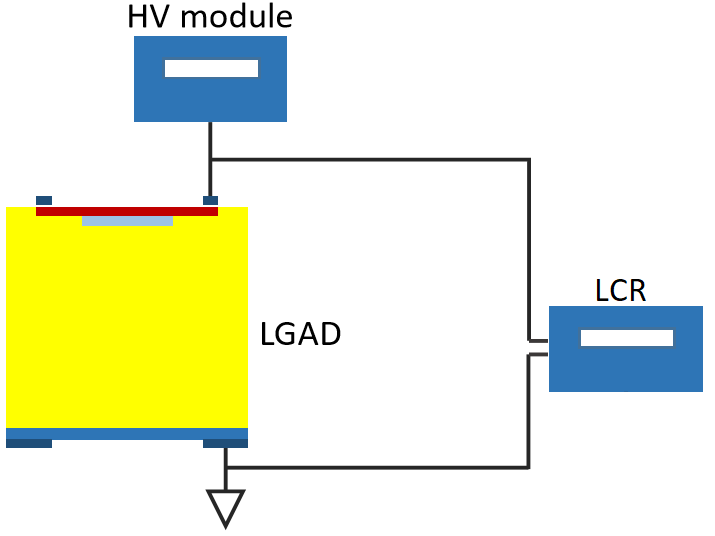
\includegraphics[width=10.0cm]{assets/iv_cv.png}
%    \caption{Figura mostrando o diagrama para a medida de corrente e capacitância de um sensor LGAD.}
%    \label{setup1}
%\end{figure}
\thispagestyle{plain}
Inicialmente será construída uma bancada de testes capaz de medir a corrente de fuga e a capacitância em função da voltagem aplicada ao sensor. Em maiores detalhes, a montagem será composta por uma estação de prova onde os sensores serão acomodados durante os testes. Uma fonte de alta tensão com resolução para a medida de corrente será utilizada para aplicar a tensão e medir a corrente de fuga dos sensores. A medida da capacitância do LGAD será feita por intermédio de um analisador LRC o qual permitirá medir a capacitância do sensor em função do bias aplicado. Por fim, todos esses equipamentos serão controlados por um programada de controle e aquisição dos dados o qual será produzido em ambiente LabView para monitorar as medidas e controlar sua qualidade.

Um segundo setup dedicado será construído para medir o ganho dos sensores e a sua uniformidade. Nesta montagem será utilizado um laser vermelho de 660nm de pulso rápido - da ordem de pico segundos - o qual irá incidir na base do sensor produzindo elétrons de deriva devido à ionização do meio. Em seguida os elétrons serão coletados pelo campo elétrico presente na região de depleção do detector indo em direção à região de amplificação do dispositivo onde serão multiplicados. O sinal produzido neste processo será coletado no anodo e subsequentemente amplificado por intermédio de um amplificador externo sendo digitalizado em um osciloscópio. Finalmente, a carga coletada será medida através da integral da forma de onda fornecendo o valor do ganho do sensor. A uniformidade do sensor será medida com o mesmo princípio, por intermédio de uma varredura da posição de incidência do laser sobre a região sensível do sensor.

\thispagestyle{plain}
Por fim, para completar o conjunto de técnicas necessárias, a montagem de um sistema de medida precisa de tempo será feita para caracterizar os sensores em termos de sua resolução temporal. Para tanto serão necessários a utilização de uma fonte $\beta$ de $^{90}$Sr, um detector para atuar como trigger - o qual pode ser um detector Cherenkov de quartzo acoplado a um Silicon Photo Multiplier (SiPM) com resolução temporal de 10ps, ou outro sensor LGAD - e placas com eletrônica para acomodar o sensor e efetuar a leitura dos dados. Neste arranjo o trigger será colocado atrás do LGAD, tornando possível medir apenas partículas com energia suficiente para atravessar o sensor. Neste sistema o trigger também será lido por um osciloscópio, e a resolução temporal será extraída da diferença entre a distribuição de tempo medida com o LGAD e o detector trigger.

%\begin{figure}
%    \centering
%    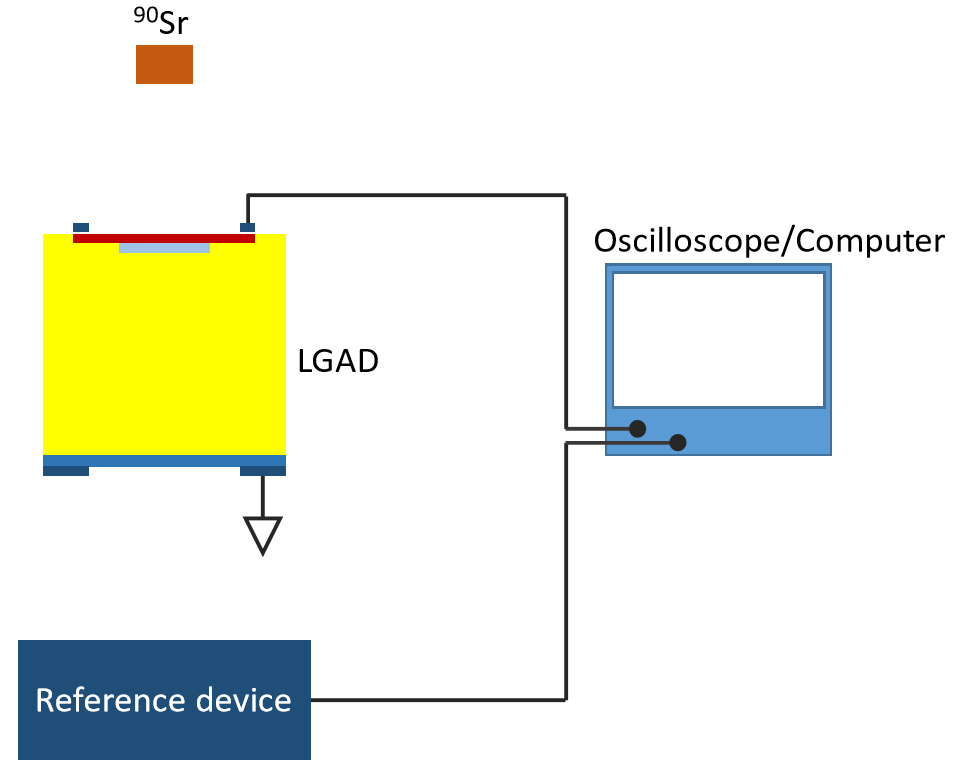
\includegraphics[width=10.0cm]{assets/time.png}
%    \caption{Figura mostrando o diagrama para a medida da resolução temporal de um sensor LGAD.}
%    \label{setup2}
%\end{figure}

Com as três técnicas experimentais estabelecidas para a medida da:

\begin{itemize}
\item Corrente de fuga
\item Ganho e uniformidade do ganho
\item Resolução temporal 
\end{itemize}
será possível diagnosticar com precisão a qualidade dos sensores LGAD. Neste ponto, cabe ressaltar que o controle de temperatura é um componente importante para todas as técnicas de medida descritas anteriormente, e desse modo um controlador de temperatura será utilizado para estabilizar a temperatura do LGAD à -30$^{\circ}$ durante todas as medida que serão efetuadas, sendo essa a temperatura de operação nominal do HGTD \cite{tdr}.

\thispagestyle{plain}

Subsequentemente, cabe destacar que o grupo HEPIC possui conhecimento adquirido ao longo de anos de pesquisa dedicada a instrumentação que serão essenciais para o desenvolvimento deste projeto em sua fase inicial, tais como: design e confecção de placas eletrônicas para sensores, desenvolvimento de {\it Front End Electronics}, desenvolvimento de {\it Back End Electronics}, i.e firmware para aquisição de dados, e desenvolvimento de software para aquisição e análise de dados. Essas ferramentas aliadas à experiência do pesquisador responsável desta proposta com o desenvolvimento de instrumentação científica \cite{tpcNIM,discharge_paper,GSI_REPO,THGEM} e com a colaboração com outros centros de pesquisa dentro da colaboração ATLAS será importante para estabelecer de forma rápida as técnicas descritas anteriormente, garantindo a qualidade dos resultados obtidos e o sucesso dos investimentos feitos para pesquisa e desenvolvimento desses sensores. 
\thispagestyle{plain}

%3 - Desafio de melhorar o sensor LGAD
Uma vez consolidada os experimentos descritos acima para a caracterização dos sensores LGAD, o passo seguinte será continuar com o desenvolvimento do dispositivo, e com base nos dados coletados buscar discutir e optimizar os parâmetros do sensor com o objetivo de produzir novas gerações de LGAD com melhores características em termos de ganho, resolução temporal, uniformidade e resistência à radiação. 

\thispagestyle{plain}
Como dito anteriormente, o programa de pesquisa proposto neste projeto será em grande parte baseado na interação com a colaboração ATLAS, de modo que teremos acesso aos recentes avanços obtidos no desenvolvimento do LGAD, tais como a identificação de vulnerabilidades presentes na geometria do sensor e a inativação do material dopante devido ao dano radioativo, os quais serão também tópicos para investigação neste projeto.

Com relação à geometria do LGAD, no atual estágio de desenvolvimento foi possível identificar fragilidades em seu design relacionados com regiões suscetíveis à ocorrência de descargas elétricas presentes nas bordas do sensor, onde o campo elétrico aplicado é mais elevado. Essa vulnerabilidade afeta a estabilidade elétrica do sensor, e essa questão será atacada no desenvolvimento dos próximos protótipos através de melhorias em seu {\it layout} as quais diminuam o campo elétrico em regiões críticas do sensor \cite{tdr}.  
\thispagestyle{plain}
   
Subsequentemente, outro aspecto importante, o ganho em um detector LGAD é uma característica que depende diretamente do perfil da concentração de dopante presente na camada de multiplicação do sensor. Devido a presença dessa camada de amplificação o sensor torna-se mais complexo e mais suscetível à danos radioativos, uma vez que a inativação do dopante e a subsequente redução de sua concentração na camada de multiplicação pela incidência de radiação provocam a redução do ganho e perdas na resolução em tempo. Para superar essa limitação, tentativas preliminares demonstraram que a adição de outros elementos de forma intersticial na rede cristalina, tais como carbono, em conjunto com o material dopante podem minimizar o impacto do dano radioativo tornando os sensores mais resistentes à radiação ionizante, entretanto com a contrapartida de diminuir a resolução em tempo \cite{tdr}. 

Com a diminuição do ganho, ocorre um aumento da corrente consumida pelo dispositivo LGAD, o que por sua vez provoca o aumento na potência dissipada. Esse fator influencia o projeto de vários outros componentes que farão parte do detector para que seja possível dimensioná-los de forma adequada para comportar a carga de calor produzida pelo dispositivo. Estas questões  demonstram a grande importância de um estudo detalhado desses aspectos durante a fase de pesquisa e desenvolvimento do sensor. %Até o momento os requisitos para a potência dissipada do dispositivo LGAD estão em aberto e serão abordados na produção dos próximos protótipos.

Como fica claro, o design do LGAD encontra-se em seu estágio inicial de desenvolvimento, e desse modo inúmeras oportunidades para contribuição intelectual estão em aberto para serem exploradas na próxima fase da pesquisa e desenvolvimento que está para ser iniciada.% De forma objetiva, o cronograma do projeto prevê a produção de dois lotes de dispositivos destinados à fabricação de protótipos para o início na segunda metade de 2020. Subsequentemente, o mesmo irá se estender até o início 2021, afim de validar as possíveis modificações adotadas com relação ao {\it layout}, materiais empregados e diversos componentes e processos que serão empregados na produção dos dispositivos. Isso é essencial para assegurar que pontos importantes em relação ao sensor e sua integração sejam revisados e verificados de modo a atender as especificações requeridas pelo experimento ATLAS.

\thispagestyle{plain}
Por conseguinte, uma vez que todos os desafios técnicos forem superados, com o sensor e os fabricantes definidos, será iniciada a fase de fabricação dos dispositivos. Neste período a experiência adquirida durante a fase de desenvolvimento será fundamental para criar os procedimentos e protocolos requeridos com o objetivo de minimizar a probabilidade dos sensores apresentarem falhas durante a operação no experimento. %Novamente, o grupo HEPIC e o pesquisador responsável participarão desta fase na criação das especificações para os sensores e os devidos protocolos para os testes.     

% FASE 3 -  
%4 - Desafio de aplicar para a medida de raios-x
Paralelamente à todas as atividades dedicadas ao desenvolvimento do LGAD em conjunto com a colaboração ATLAS, outros objetivos relacionados com a aplicação para a detecção de raios-X também serão somados a este projeto. Devido às excelentes características apresentadas, as quais incluem sua alta eficiência quântica para uma ampla faixa de comprimentos de onda \cite{book1,book2}, sensores semicondutores de diversos tipos são amplamente empregados na detecção de raios-X em experimentos que utilizam luz síncrotron. Com a vantagem de possuírem ganho intrínseco, dispositivos LGAD permitem a detecção de raios-X de baixa energia bem como a detecção de sinais produzidos por poucos fótons, sendo desta forma muito flexível. 

%Com isso em mente, através da colaboração com o Laboratório de Sistemas Integráveis (LSI) da Escola Politécnica da USP será possível produzir sensores LGAD e modificar o seu perfil de dopagem de modo a produzir dispositivos com ganho adequado para operar no regime de avalanche proporcional optimizados para a detecção de raios-X. Por conseguinte, os dispositivos serão testados de forma rigorosa com os mesmos critérios aplicados aos sensores destinados para a colaboração ATLAS. Isso será um passo importante para estabelecer o domínio da tecnologia e a autossuficiência com respeito à produção desses dispositivos para aplicações no Brasil.

% CONSIDERACOES FINAIS

Por fim, esta proposta de projeto tem como objetivos estratégicos de curto prazo preparar os experimentos necessários para o desenvolvimento do LGAD no CERN/ATLAS, e por conseguinte colaborar com o experimento ATLAS na construção do HGTD. E para médio e longo prazo os objetivos de desenvolver dispositivos semicondutores para diversas aplicações científicas no âmbito nacional e internacional, e com isso consolidar a tecnologia de sensores semicondutores.

 %varios milestones estabelecidos

%Outro aspecto fundamental   

%Como descrito anteriormente, o ganho em um detector LGAD depende diretamente do perfil da concentração do dopante presente na camada de multiplicação do sensor. Dessa forma, o fator que mais contribui para o dano radioativo em sensores LGAD é a remoção e subsequente redução da concentração de dopante na camada de multiplicação o que por conseguinte provoca a redução do ganho e perdas na resolução em tempo. Com o R&D desenvolvido ate o momento, 

%preliminares demonstram que a adição de outros materiais, tais como carbono, junto com o material dopante podem minimizar o impacto do dano radioativo tornando os sensores mais resistentes à radiação ionizante, entretanto mais estudos devem ser conduzidos para compreender os fatores limitantes obtidos com a adição de outros materiais.


%incluindo a sua produção no Brasil. Vários pesquisadores que integram a equipe deste projeto vêm de outros grupos de pesquisa da USP, do IPEN, conferindo-lhe um forte carácter interdisciplinar, essencial no desenvolvimento de aplicações tanto em imagem de raios X, como na detecção de nêutrons.









\chapter{Cronograma de execução do projeto}

Como ilustra a seta em amarelo na Fig. \ref{crono}, este projeto terá a duração de um ano com início em 2021 e término em 2022, e estará focada na construção e teste do protótipo do HGTD. 

O plano de execução para o desenvolvimento do LGAD, mostrado na Fig. \ref{crono}, tem a duração total de cinco anos (2020 - 2025), onde estão inclusas as fases de desenvolvimento do sensor - início de 2020 até o início de 2022 - e produção dos dispositivos LGAD, de 2022 até 2024. 
\thispagestyle{plain}

Além das atividades de desenvolvimento do LGAD, durante este período o cronograma também prevê a construção do HGTD (\textit{demonstrator}), e a sua caracterização com raios cósmicos e raios-X. Essas duas fases são importantes pois permitirão o desenvolvimento das atividades relacionadas com a construção do HGTD, a caracterização de seus diversos componentes, bem como a sua integração com a eletrônica de aquisição de dados, corroborando com os objetivos propostos neste documento. 

\begin{figure}[H]
    \centering 
    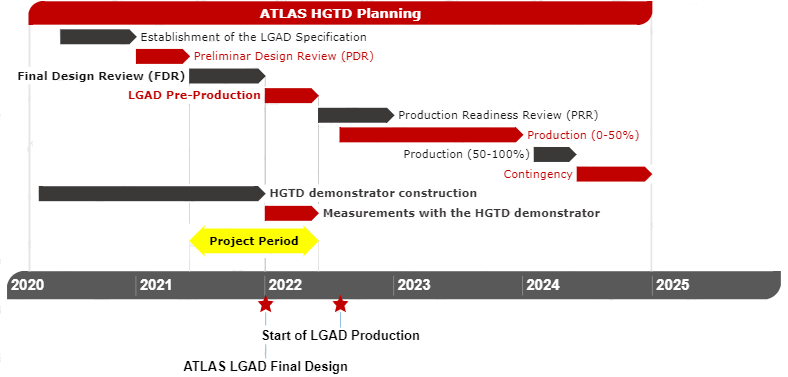
\includegraphics[width=16.0cm]{assets/cronogama.png}
    \caption{Figura mostrando o planejamento para o desenvolvimento do LGAD e HGTD, incluindo as revisões do projeto (PDR, FDR, PRR), pré-produção e produção. Os principais {\it milestones} do projeto são mostrados em sua linha do tempo.}
    \label{crono}
\end{figure}

\renewcommand{\cleardoublepage}{}
\renewcommand{\clearpage}{}
\chapter{Importância científica do projeto}

\thispagestyle{plain}
Uma vez que este projeto está relacionada com a detecção de radiação ionizante, essa proposta possui um grande potencial de inovação científico-tecnológica, e poderá dar origem a diversos sensores, ampliando a propriedade intelectual dos processos e dispositivos produzidos. Além disso, o pesquisador responsável por essa proposta possui experiência no desenvolvimento de instrumentação para física de altas energias, adquirida através do trabalho realizado no projeto de {\it upgrade} do TPC do experimento ALICE no CERN \cite{tpcNIM,discharge_paper,GSI_REPO,THGEM}, isso somado à infraestrutura presente no laboratório do HEPIC do Instituto de Física da Universidade de São Paulo para o desenvolvimento de instrumentação nuclear, permitirá a transferência total de tecnologia relacionada com sensores semicondutores de alta performance para o grupo, bem como ageração de novas tecnologias e aplicações, permitindo consolidar a linha de pesquisa em sensores semicondutores no Departamento de Física Nuclear do Instituto de Física da USP. Esse projeto irá corroborar com programas experimentais atualmente em andamento no grupo relacionado com a espectroscopia e reconstrução de imagens com raios-X \cite{THGEM,NIM,xray}, ampliando a capacidade tecnológica do HEPIC com respeito à detecção de radiação ionizante. 
\thispagestyle{plain}

A vista disso, no âmbito nacional, com as ferramentas criadas neste projeto será possível colaborar com os programas de instrumentação em diversos programas de pesquisa presentes no Brasil tais como o Laboratório Nacional de Luz Síncrotron (LNLS), no que diz respeito ao desenvolvimento de sistemas de detecção. De acordo com os estudos levantados pelos pesquisadores do Sirius e descritas em seu projeto \cite{sirius}, {\it 'existe hoje no Brasil uma oportunidade excepcional para o desenvolvimento de expertise na área de detectores híbridos, visando atender às exigências das linhas de luz do Sirius. Futuramente, essa experiência poderá resultar em desenvolvimentos para as áreas médica, industrial e educacional'}. Isso está alinhado com os objetivos desta proposta.

\thispagestyle{plain}
No final do projeto, o {\it know how} adquirido na linha de pesquisa com sensores semicondutores estará consolidado e pronto para dar continuidade ao trabalho independente deste grupo em novas aplicações bem como na geração de novas tecnologias.

\renewcommand{\cleardoublepage}{}
\renewcommand{\clearpage}{}

\begin{thebibliography}{9}

\bibitem{HL_LHC} Oliver Brüning and Lucio Rossi, The High Luminosity Large Hadron Collider: The New Machine for Illuminating the Mysteries of Universe, World Scientific, CERN, October 2015,  https://doi.org/10.1142/9581

\bibitem{tdr} ATLAS collaboration, Technical Proposal: A High-Granularity Timing Detector for the ATLAS Phase-II Upgrade, CERN-LHCC-2018-023.

\bibitem{JIN_LGAD} N. Moffat. et al., JINST. 13, (2018) C03014.

\bibitem{NIMA_LGAD} M. Carulla. et al., Nucl. Instrum. Meth. A 924, (2019) 373. 

%
\bibitem{NIMA_LGAD_I} G. Pellegrini. et al., Nucl. Instrum. Meth. A 831, (2016) 24-28.

\bibitem{NIMA_LGAD_II} D. Breton. et al., Nucl. Instrum. Meth. A 835, (2016) 51-60.

\bibitem{NIMA_LGAD_III} M. Ferrero. et al., Nucl. Instrum. Meth. A 919, (2019) 16-26.
%

\bibitem{atlas_rev} G. Brandt, \textit{Review of Current Standard Model Results from ATLAS}. Few-Body Syst 59, 128 (2018). 

%%
%\bibitem{IPEN_REATOR} I. A. Tomiyoshi, S. S. Iyer, and C. Rodrigues, Journal of Radioanalytical and Nuclear Chemistry, 237, 1-2, (1998) 85-89.

%\bibitem{IPEN_AURORA} C.B.R. Parente. et al., Nucl. Instrum. Meth. A 622, (2010) 678–684.

%%
%\bibitem{ALICEUP} ALICE Collaboration, J. Phys. G: Nucl. Part. Phys. 41 (2014) 087001.

%\bibitem{ref1} B. A. et al. (ALICE Collaboration), Technical design report for the upgrade of the alice time projection chamber, CERN-LHCC-2013-020 A886 (2013), http://cds.cern.ch/record/1622286.


\bibitem{tpcNIM} M.M. Aggarwal, et al., Nucl. Instrum. Meth. A 903, (2018) 215–223. 

\bibitem{discharge_paper} A. Deisting, et al., Nucl. Instrum. Meth. A 937, (2019) 168–180.


%
\bibitem{GSI_REPO} Garabatos C., et al., Stability test of ALICE TPC GEM chambers at the LHC, GSI FAIR SCIENTIFIC REPORT 2017, DOI:10.15120/GSI-2017-01856.
%

\bibitem{THGEM} H. Natal da Luz, et al., EPJ Web of Conferences 174, (2018) 01012.

%\bibitem{book1} G. Lutz, Semiconductor Radiation Detectors: Device Physics, Springer-Verlag, Berlin Heidelberg, 2007. 

%\bibitem{book2} H. Spieler, Semiconductor Detector Systems, Oxford University Press, Great Britain, 2005.

%\bibitem{COMSOL} https://www.comsol.com/comsol-multiphysics

\bibitem{NIM} G. G. A. de Souza and  H. Natal da Luz, Nucl. Inst. Meth. A 937, (2019) 141–147.
\thispagestyle{plain}
\bibitem{xray} G.G.A. de Souza and H.N. da Luz, X-Ray Spectrometry 48, 5 (2018).

\bibitem{sirius} https://www.lnls.cnpem.br/sirius/livro-projeto-sirius/
\thispagestyle{plain}

%\bibitem{production_protocol} http://indico.cern.ch/event/645829/


\end{thebibliography}
\newpage

\end{document}
